\documentclass{entcs}
\usepackage{entcsmacro}
%NOTE: oz.sty clashes with entcs.cls, so we use a hacked version of oz.sty
\usepackage{czt}
\usepackage{graphicx}

% Extra general macros for this paper.

% Extra math-mode macros for this paper.
% Some of these may eventually go into czt.sty
\newcommand{\V}{\mathcal{V}}
\newcommand{\Zc}{Z_C}
\newcommand{\sexprUnfoldsTo}{\mathrel{=_{se}}}
\newcommand{\declListUnfoldsTo}{\mathrel{=_d}}
\newcommand{\unprefix}{\mathrel{unprefix}}
\newcommand{\schemaEquals}{\mathrel{=_S}}

\def\lastname{Utting, Malik, Toyn}

\begin{document}
\begin{frontmatter}
  \title{Transforming Z with Rules}
  \author{Mark Utting\thanksref{emailMark}}
  \address{Department of Computer Science\\
    The University of Waikato\\
    Hamilton, New Zealand} 
  \author{Petra Malik\thanksref{emailPetra}}
  \address{Department of Computer Science\\
    The University of Waikato\\
    Hamilton, New Zealand} 
  \author{Ian Toyn\thanksref{emailIan}}
  \address{Department of Computer Science\\
    The University of York\\
    Heslington, York, UK}
  \thanks[emailMark]{Email: \texttt{marku@cs.waikato.ac.nz}}
  \thanks[emailPetra]{Email: \texttt{petra@cs.waikato.ac.nz}}
  \thanks[emailIan]{Email: \texttt{ian@cs.york.ac.nz}}
\begin{abstract}
  This paper describes a simple extension of Z that allows transformation
  and reasoning rules to be written in a natural, Z-like notation.  This
  gives a high-level, declarative way of specifying transformations of Z
  terms, which makes it easier to build new Z manipulation tools.
  We describe the syntax and semantics of these rules, plus several reasoning
  engines that use sets of rules to manipulate Z terms.  We demonstrate the
  utility of rules by discussing one set of rules that defines schema
  unfolding of the schema expressions in Z and another set that is used by
  the ZLive animator to preprocess Z expressions into a form more suitable
  for animation.  
\end{abstract}
\begin{keyword}
  Z, CZT, reasoning, rewriting rules
\end{keyword}
\end{frontmatter}



\section{Introduction}

In many Z tools, schema unfolding and other Z transformations are performed
by large amounts of low-level code (for example, in C or Java) that
manipulate the syntax of Z schema expressions and return equivalent
unfolded terms.  This low-level approach is error-prone, and the code that
performs the transformations is time-consuming to write and difficult to
read.  The problem is that the essence of the abstract transformations are
hidden in the masses of low-level code.

This means that building new Z transformation tools is time-consuming,
requires programming skills, and also requires detailed knowledge of the
API for manipulating Z syntax trees.  In contrast, in an ideal world, it
should be quick and easy to define new Z transformations by writing them in
the Z notation itself, in a high-level, declarative style that is easily
understood and can perhaps even be proven correct according to some given Z
logic.  A high-level notation such as this gives better support for the
capture and reuse of the knowledge implicit in the
rules~\cite{armour:business-model00}.

This paper proposes such a declarative notation, called ZedRules.
It is an extension of the standard Z notation that provides \emph{jokers}
that can stand for arbitrary expressions, predicates, declarations etc.
It allows equality and inference rules to be written in a Z-like notation,
and users can extend this notation by defining new operators within Z.

Section \ref{sec:syntax} describes the syntax and semantics of the
ZedRules.  Section~\ref{sec:tools} describes three different reasoning
engines provided by CZT to use the rules.  Section~\ref{sec:schemas} shows
how the rules can be used to specify unfolding and normalisation of schema
expressions and Section~\ref{sec:zlive} shows some of the rules that are
used by ZLive to preprocess Z expressions and predicates.



\section{Related Work} \label{sec:relwork}


\section{Rule Syntax and Semantics} \label{sec:syntax}

This section describes the syntax and semantics of the Z rules.

Each rule has a single conclusion and possibly several antecedents, so is a
horn clause.  Thus we have a high-level Prolog-like notation (but with Z
syntax) for defining Z transformations and automatic proofs.

We describe the semantics of the rules independently of any operational
description of how rules can be used. 

This allows rules to be used by many different reasoning and rewrite
engines.  Each engine may place different restrictions on the rules
that it allows, may apply rules using a different semantics (apply once,
apply exhaustively, apply to all subterms bottom-up or top-down etc.), and
may use a different implementation technology (for example, an interpreter
that applies the rules or a compiler that transforms the rules into Java
code).


\section{Tools for Rules} \label{sec:tools}

To use and test the rules, several tools have been implemented.

\subsection{A Simple Interactive Prover}

\begin{figure}[htbp]
  \centering
  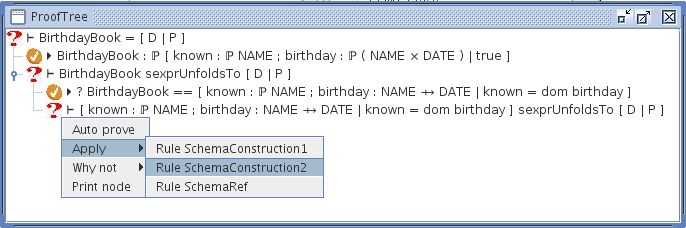
\includegraphics[width=\textwidth]{cztprover1}
  \caption{Screenshot of Interactive Prover}
  \label{fig:cztprover}
\end{figure}

The simple interactive prover shown in figure~\ref{fig:cztprover} is
used as a debugging aid.  It displays an entire proof tree in tree
form.  Each node is labelled with a subgoal, which is either a sequent
(predicate) or a proviso.  Each node can be closed (proven), indicated
by a tick icon, or open (not proven), indicated by a question mark
icon.

The user can manipulate the proof tree by applying rules to sequents,
undoing rule applications, or requesting a proviso to be checked.
Clicking on a node will popup a menu offering the choices available
for that particular node.  For a proviso that has not yet been
checked, for example, a menu entry for requesting the check is
offered.  If the check succeeds, this node is considered closed and
the icon will change from a question mark to a tick.

The menu for sequents to which no rule has been applied yet offers the
choice of ``Auto prove'' this sequent or to apply one of the matching
rules.  It also has a ``Why not'' submenu, which lists all the rules
that cannot be applied.  By selection one of those, the user gets
detailed debugging information why the unification of the selected
sequent and the conclusion of a particular rule failed.

To provide the submenus ``Apply'' and ``Why not'', the prover goes
through all the known rules and tries to apply them to the current
sequent.  If this test rule application suceeds, the corresponding
rule name gets added into the ``Apply'' submenu; if it fails, the rule
name gets added into the ``Why not'' submenu.  While this approach
might be too inefficient and slow for large rule sets, it has shown to
be very helpful for our purposes.

The ``Auto prove'' menu entry, provided for sequents to which no rule
has been applied, calls the automated prover described in the next
section.  If a proof is found, the resulting proof tree is displayed
as a subtree of the current node and the user can browse and
manipulate it.  Browsing a proof tree is eased by allowing subtrees to
be hidden.  If the pointer is above a particular node, the tooltip
gives information about whether and which rule has been applied, or
whether the current node is a proviso.

\subsection{An Automated Depth-First Prover}

A simple depth-first prover is used to find proofs automatically.
Given a predicate, it tries to apply the rules in the order they
appear in the Z specification.  If a rule application succeeds, a
sequence of new subgoals is created and attempted to be proven next
(in the order provided by the rule).  If proving the new subgoals
fails, the next rule is tried instead.

If a subgoal is a proviso, it is checked and changes into one of three
states: \emph{PASS} (the side-condition was correctly discharged),
\emph{FAIL} (the side-condition is false), \emph{UNKNOWN} (the
side-condition needs to be checked later, when the sequent is
instantiated more fully).  The current implementation treats state
\emph{UNKNOWN} the same as \emph{FAIL}, thus relies on the order of
subgoals provided by the rule writer.

Note that the simple prover uses a shallow backtracking algorithm and
therefore might fail to find a proof even when there exists one.  If a
proof for a subgoal is found, the prover sticks to it and no attempt
is made to find an alternative proof.  This might prevent another
subgoal from being proven.  Even though this approach is less general
than deep backtracking, this has not been a problem for the rules used
so far.  Furthermore, if a proof is found using shallow backtracking,
it is usually found more quickly than using deep backtracking.

\subsection{A Rewrite Engine}

The purpose of the rewrite engine is to rewrite a given Z term using a
given set of rewrite rules.  A rewrite rule is a rule whose conclusion
is of a particular form and consists of a left side (which needs to
match the term to be rewritten) and a right side (which represents the
result of the transformation).  For example, a Z expression~$e1$ is
rewritten to the Z expression~$e2$ if $e1 = e2$ can be proven using
the given rewrite rules.

Usually, the task is to compute $e2$ for a given Z expression $e1$.
To do that, the rewrite engine asks the prover to prove $e1 = E$,
where $E$ is an expression joker.  The rewrite rules should be
designed so that, if a proof is found, the right hand side of the
equation is ground, i.e.\ does not contain any unbound jokers.  Then
$e1$ is substituted by, or rewritten to, $e2$.

Currently, there are methods for rewriting an expression (using $e1 =
e2$ rules) and a predicate (using $p1 \leftrightarrow p2$ rules) once.
However, there are endless ways of combining rewrites into sequences
of rewrites.  Subterms can be considered, either in a bottom-up or a
top-down approach.  The current implementation rewrites each level of
a term in a top-down manner.  A term is rewritten until it does not
change any more, and then the subterms are rewritten in the same way.

\section{Example Rules: Schema Unfolding} \label{sec:schemas}

\begin{zsection}
  \SECTION unfold \parents zpattern\_toolkit, standard\_toolkit
\end{zsection}

This Z section contains rules for unfolding and normalising declarations
and schema expressions.  For example, given a schema expression such as 
$E \land [x:\nat | p~x]$ where $E$ is the name of a schema, these rules
define a normalisation process that will transform this schema expression
into something of the form $[D|P]$, where $D$ is a list of variable
declarations whose types are all base types and $P$ is a predicate that
will contain constraints like $x \in \nat$ and $p~x$.

We start by declaring the jokers used in all the rules in this section.

\begin{zedjoker}{DeclList} D, D1, D2, D3, D4, D5 \end{zedjoker}
\begin{zedjoker}{Pred} P, P1, P2, P3, P4, P5 \end{zedjoker}
\begin{zedjoker}{Expr} E, E1, E2, E3, E4, E5 \end{zedjoker}
\begin{zedjoker}{Name} v, v1, v2, v3, v4, v5 \end{zedjoker}

To clearly distinguish our rules for unfolding declaration lists and
schema expressions from other rules, we introduce two new infix
operators: $\sexprUnfoldsTo$ and $\declListUnfoldsTo$.  
We do not really need to define their semantics in order to use them within
rules, but to reassure readers, we define their semantics to be just
equality.  In fact, the intention is that the right hand argument
will be the unfolded and normalized form of the left hand argument.

\begin{verbatim}
%%Zinword \sexprUnfoldsTo sexprUnfoldsTo
%%Zinword \declListUnfoldsTo declListUnfoldsTo
\end{verbatim}

\begin{zed}
  \relation ( \_ \sexprUnfoldsTo \_ )
\end{zed}
\begin{zed}
  \relation ( \_ \declListUnfoldsTo \_ )
\end{zed}


\begin{gendef}[SCHEMA]
  \_ \sexprUnfoldsTo \_ : SCHEMA \rel SCHEMA \\
  \_ \declListUnfoldsTo \_ : SCHEMA \rel SCHEMA
\where
  \forall s1,s2:SCHEMA @ s1 \sexprUnfoldsTo s2 \iff s1=s2 \\
  \forall s1,s2:SCHEMA @ s1 \declListUnfoldsTo s2 \iff s1=s2 \\
\end{gendef}


\subsection{Unfolding Declaration Lists}

We use the $\declListUnfoldsTo$ operator for unfolding declaration
lists.   The left-hand side is always of the form $[DeclList|true]$
and the right-hand side (which is usually a generated output) is
of the form $[D|P]$, where the declaration list $D$ has no duplicated
names and all its types are Z base types, and the predicate $P$
contains any additional typing constraints that were in DeclList.

The next few rules specify the $\declListUnfoldsTo$ operator.
The rules are intended to recurse through a declaration list from left
to right, with the base case of an empty declaration list being handled
by the EmptyDeclList rule.  Note that multiple declarations such as
$x,y,z:T$ are expanded out into separate declarations before rules
are applied, so the rules that follow cover all possible kinds
of declarations.

The VarDecl1 rule is a special case of VarDecl2, which applies when $E$ is
already a base type.  Since VarDecl1 comes before VarDecl2 in this file,
the rewrite tactic gives it higher priority, and this avoids introducing
redundant tautologies (such as $E \in \arithmos$, which is guaranteed to
be true by the type system) into the predicate.  This is an example of
how we can influence the behaviour of the rewrite tactic by placing more
specific rules before more general ones.  Of course, in the interactive
prover, the user could choose to apply either rule when $E$ is a base type.

\begin{zedrule}{VarDecl1}
   \proviso E : \power E \\
   [D1 | true] \declListUnfoldsTo [D2 | P2]
\derives
   [v:E; D1 | true] \declListUnfoldsTo [v:E; D2 |  P2]
\end{zedrule}

\begin{zedrule}{VarDecl2}
   \proviso E : \power E2 \\
   [D1 | true] \declListUnfoldsTo [D2 | P2]
\derives
   [v:E; D1 | true] \declListUnfoldsTo [v:E2; D2 |  v \in E \land P2]
\end{zedrule}

\begin{zedrule}{ConstDecl}
   \proviso E : E2 \\
   [D1 | true] \declListUnfoldsTo [D2 | P2]
\derives
   [v==E; D1 | true] \declListUnfoldsTo [v:E2; D2 |  v = E \land P2]
\end{zedrule}

This rule creates a subgoal $E \sexprUnfoldsTo \ldots$ that will
invoke the schema expression rules in the next section.  So the
two sets of $\declListUnfoldsTo$ and $\sexprUnfoldsTo$ rules are
mutually recursive.

\begin{zedrule}{IncludeDecl}
   E \sexprUnfoldsTo [D1 | P1] \\
   [D | true] \declListUnfoldsTo [D2 | P2] \\
   \proviso [D1 | true] \land [D2 | true] : \power [D3]
\derives
   [E; D | true] \declListUnfoldsTo [D3 |  P1 \land P2]
\end{zedrule}

\begin{zedrule}{EmptyDeclList}
   [~ | true] \declListUnfoldsTo [~ | true]
\end{zedrule}


\subsection{Unfolding Schema Expressions}

This section defines the unfolding of schema expressions,
using the $SE \sexprUnfoldsTo STEXT$ operator, where $SE$
is a schema expression and $STEXT$ is the resulting normalized
schema construction ($[Decls|Preds]$, where the types in $Decls$
are only base types).

Top-level schema expressions are unfolded into schema construction
expressions, which can then be expanded into sets of bindings.
However, we have a special case for $\exists$, so that we can
put all the variables into the bound variable list of the
set comprehension, then create a binding using a subset of
those variables.  Putting all the variables at the same level
of scope gives the evaluation optimization algorithms more
freedom to reorder things later.

\begin{zedrule}{TopLevel}
  \proviso E : \power [D2] \\
  E  \sexprUnfoldsTo [D | P]
\derives
  E = [D | P]
\end{zedrule}

\begin{zedrule}{Theta}
  \proviso E : \power [D] \\
  \proviso E2 == \theta [D | true]
\derives
  \theta E = E2
\end{zedrule}

NOTE: we need thirteen versions of this next rule -- one for
each possible decoration.   In the future we will add
support for Stroke-List jokers, so that all decorations can
be handled by a single rule.

\begin{zedrule}{ThetaPrime}
  \proviso E : \power [D] \\
  \proviso E2 == \theta [D | true] '
\derives
  \theta E~' = E2
\end{zedrule}

\begin{zedrule}{SchemaConstruction1}
  [D1 | true] \declListUnfoldsTo [D2 | true]
\derives
  [D1 | P] \sexprUnfoldsTo [D2 | P]
\end{zedrule}

\begin{zedrule}{SchemaConstruction2}
  [D1 | true] \declListUnfoldsTo [D2 | P2]
\derives
  [D1 | P] \sexprUnfoldsTo [D2 | P2 \land P]
\end{zedrule}

\begin{zedrule}{SchemaRef}
  \proviso ?~ E == E2 \\
  E2 \sexprUnfoldsTo [D2 | P2]
\derives
  E \sexprUnfoldsTo [D2 | P2]
\end{zedrule}

This rule unfolds any remaining $\Delta$ schemas.
If the specification explicitly defined the $\Delta$ schema,
then the above SchemaRef rule would have unfolded it.

\begin{zedrule}{DeltaRef}
  \proviso v2 == \Delta \unprefix v \\
  [v2; v2~'] \sexprUnfoldsTo [D1|P1]
\derives
  v \sexprUnfoldsTo [D1|P1]
\end{zedrule}

This rule unfolds any remaining $\Xi$ schemas.
If the specification explicitly defined the $\Xi$ schema,
then the above SchemaRef rule would have unfolded it.

\begin{zedrule}{XiRef}
  \proviso v2 == \Xi \unprefix v \\
  [v2; v2~'] \sexprUnfoldsTo [D1|P1] \\
  \proviso [v2|true] : \power [D2]
\derives
  v \sexprUnfoldsTo [D1|P1 \land \theta [D2|true] = \theta [D2|true]~']
\end{zedrule}

NOTE: we also currently need thirteen versions of this next rule 
-- one for each possible decoration. 

\begin{zedrule}{SchemaPrime}
   E \sexprUnfoldsTo [D1 | P1] \\
   \proviso [D2|P2] == [D1|P1]~' \\
\derives
   E~' \sexprUnfoldsTo [D2 | P2]
\end{zedrule}

The type proviso in the ExistsSchema rule checks
that $D1$ and $D2$ are type compatible.  The $\schemaminus$
operator in the proviso calculates $D2 - D1$.  That is,
$D4$ will contain all the declarations that appear in $D2$
but do not appear in $D1$. 

\begin{zedrule}{ExistsSchema}
   [D|P] \sexprUnfoldsTo [D1 | P1] \\
   E2 \sexprUnfoldsTo [D2 | P2] \\
   \proviso [D1 | true] \land [D2 | true] : \power [D3] \\
   \proviso [D4|true] == [D2|true] \schemaminus [D1|true]
\derives
   (\exists D | P @ E2) \sexprUnfoldsTo [D4 | (\exists D1 @ P1 \land P2)]
\end{zedrule}

The semantics of schema negation requires the schema to be
normalised before the predicate is negated.

\begin{zedrule}{SchemaNegation}
  E \sexprUnfoldsTo [D | P]
\derives
  (\lnot E) \sexprUnfoldsTo [D | \lnot P]
\end{zedrule}

\begin{zedrule}{SchemaConjunction}
  E1 \sexprUnfoldsTo [D1 | P1] \\
  E2 \sexprUnfoldsTo [D2 | P2] \\
 \proviso [D1 | true] \land [D2 | true] : \power [D3]
\derives
  (E1 \land E2) \sexprUnfoldsTo [D3 | P1 \land P2]
\end{zedrule}

\begin{zedrule}{SchemaDisjunction}
  E1 \sexprUnfoldsTo [D1 | P1] \\
  E2 \sexprUnfoldsTo [D2 | P2] \\
 \proviso [D1 | true] \land [D2 | true] : \power [D3]
\derives
  (E1 \lor E2) \sexprUnfoldsTo [D3 | P1 \lor P2]
\end{zedrule}

\begin{zedrule}{SchemaImplication}
  E1 \sexprUnfoldsTo [D1 | P1] \\
  E2 \sexprUnfoldsTo [D2 | P2] \\
 \proviso [D1 | true] \land [D2 | true] : \power [D3]
\derives
  (E1 \implies E2) \sexprUnfoldsTo [D3 | P1 \implies P2]
\end{zedrule}

\begin{zedrule}{SchemaEquivalence}
  E1 \sexprUnfoldsTo [D1 | P1] \\
  E2 \sexprUnfoldsTo [D2 | P2] \\
 \proviso [D1 | true] \land [D2 | true] : \power [D3]
\derives
  (E1 \iff E2) \sexprUnfoldsTo [D3 | P1 \iff P2]
\end{zedrule}

Schema projection, $E1 \project E2$, is similar to schema conjunction,
but the resulting schema has only the names that are declared in $E2$.
Any other names that are declared in $E1$ are hidden existentially.

\begin{zedrule}{SchemaProjection}
  E1 \sexprUnfoldsTo [D1 | P1] \\
  E2 \sexprUnfoldsTo [D2 | P2] \\
  \proviso [D1 | true] \land [D2 | true] : \power [D3] \\
  \proviso [D4 | true] == [D3 | true] \schemaminus [D2 | true]
\derives
  E1 \project E2 \sexprUnfoldsTo [D2 | (\exists D4 @ P1 \land P2)]
\end{zedrule}

To calculate the precondition of a schema, we must existentially
hide all the output names, such as $x!$ or $x'$.  The $postnames$ 
operator in the following rule takes a normalised schema as input and
returns (in $D2$) just the declarations whose names have a final decoration 
of $!$ or $'$.  These names are removed from $D4$, so that $D3$ contains 
only the declarations of names that should appear in the precondition, 
such as $x$, $x?$ and $x_2$.

\begin{zedrule}{SchemaPrecondition}
  E \sexprUnfoldsTo [D4 | P2] \\
  \proviso [D2 | true] == postnames [D4 | true] \\
  \proviso [D3 | true] == [D4 | true] \schemaminus [D2 | true] \\
\derives
  \pre E \sexprUnfoldsTo [D3 | (\exists D2 @ P2)]
\end{zedrule}

TODO: schema hiding, schema piping and sequential composition,
schema forall, schema exists unique.


\subsection{Rules for Unfolding Quantified Declarations}

When rewriting terms involving quantifiers, we want to
rewrite and expand the schema text $E$ within quantifiers
such as $\exists E @ P$ or $(\lambda E@E2)$, as well as rewriting
the predicates and expressions within the body of the quantifiers.
The rewrite tactics try to transform such schema text using the 
$\schemaEquals$ relation.  So the following rule applies the above 
schema unfolding rules to unfolding any schema text that appears within 
the bound variable part of quantifiers.
\begin{zedrule}{Quantifiers}
   [D|P] \sexprUnfoldsTo [D1|P1]
\derives
   [D|P] \schemaEquals [D1|P1]
\end{zedrule}


\subsection{Rules for Unfolding Predicates}

If a schema expression $E$ is used as a predicate, it is equivalent to
checking that $\theta E$ (a binding constructed from names that are
currently in scope) satisfies the predicate part of $E$ 
(including any subtypes in the declarations).  So this rule
transforms any expression that is used as predicate into $\theta E \in E$.
\begin{zedrule}{SchemaPred}
  E \iff \theta E \in E
\end{zedrule}


\section{Example Rules: ZLive Preprocessor} \label{sec:zlive}

\section{Conclusions} \label{sec:concl}


TODO: conclusions


In the future, we would like to be able to extend the ZedRules notation to
support a variety of Z logics, such as
$Z_C$~\cite{henson:revising-z-1-99,henson:revising-z-2-99},
$\mathcal{V}$~\cite{brien:calculus-schemas-z00} (a successor of the
$\mathcal{W}$ logic that appeared in early drafts of the Z standard).  It
is desirable to support both $Z_C$ and $\mathcal{V}$ (and any future
proposals for Z logics), since they are rather different and it would be
interesting to compare them in a common framework.  For example,
substitution is a meta-level operation in $Z_C$, but is defined within the
object logic of $\mathcal{V}$.  To supporting richer logics such as these,
it would be necessary to add a few more proviso constructs and to
generalise antecedents into sequents that can specify a different context
to that of the conclusion.  For example, an antecedent such as $x:T \vdash
P$ would allow the proof of $P$ to proceed in an extended context where the
new variable $x$ is declared and has type $T$.  This is the same 

The current CZT reasoning tools construct an explicit proof tree that
allows proofs to be recorded, replayed, displayed, checked by independent
tools etc.
It would be interesting to build a tactic layer on top of this proof
tree, using a tactic language such as ANGEL~\cite{martin:tactics}, which
has been used as the basis of several other Z provers (CadiZ, Jigsaw1,
Jigsaw2, Ergo).  This would make it easier to program combinations of rules
in flexible ways, whereas currently such tactics must be written in Java.

If ZedRules was extended in both of the above ways (to support richer
logics and to provide tactics), it could be used as a general Z theorem
prover.  However, we do not have any plans to do this, for three reasons:
\begin{enumerate}
\item There are already several other good theorem provers for Z, so
  developing another would simply fragment the existing small user-base
  further.
\item For practical theorem proving, it is necessary to develop a large set
  of rules (several for each Z construct), derived rules and tactics to
  automate the common styles of reasoning.  Experience shows that this
  requires several person years of theory development. 
\item The speed of the current CZT implementation of ZedRules is not
  sufficiently fast for practical reasoning.  The automated tactics can
  apply a few hundred rules per second, which is adequate for simple unfolding
  tasks, but not adequate for heavy-duty reasoning with lots of tactics --
  a good theorem prover needs to perform tens or hundreds of thousands of
  rules per second to be pleasant to use.
\end{enumerate}

In the future, we would also like to be able to translate the rules
into a form that existing Z theorem provers can accept, so that we can prove
rules correct and prove that a given set of rules preserves the Z
semantics.  A simple declarative semantics for rules makes this
easier to achieve.

\bibliographystyle{entcs}
\bibliography{spec,logic,thmprove,misc}
\end{document}
